\documentclass[twoside]{projektInzynierskiMS1}
\usepackage{polski}
\usepackage[utf8]{inputenc}
\usepackage{amsmath}
\usepackage{graphicx}%obrazki
\usepackage{array,etoolbox}%indeksowanie wierszy w tabelach
\preto\tabular{\setcounter{magicrownumbers}{0}}
\newcounter{magicrownumbers}
\newcommand\rownumber{\stepcounter{magicrownumbers}\arabic{magicrownumbers}}
\usepackage{multirow,tabularx}
\usepackage{etoolbox}
\usepackage{float}%obrazki na tej samej stronie
\newcounter{rowcnt}
\newcommand\rownum{\ifnumequal{\value{rowcnt}}{0}{\textbf{Nr.}}{\therowcnt.}\refstepcounter{rowcnt}}
\AtEndEnvironment{tabularx}{\setcounter{rowcnt}{0}}



%\drukJednostronny

%% tytuł promotor iautor (\title to komenda standardowa)
\title{Algorytm symulowanego wyżarzania - zastosowanie w rozwiązywaniu zagadnień odwrotnych}
\promotor{dr inż. Adam Zielonka}


%% każdy autor musi mieć 3 argumenty: imię nazwisko, nr albumu, opis wkładu
\autor{Kamil Kryus}{246591}
	


%Custom commands
%-------------------------------------------------------------------------------
\newcommand{\hugeFontSize}{}
\newcommand{\newLine}{~\\}
\newcommand{\si}{ś}
\newcommand{\SI}{Ś}
%-------------------------------------------------------------------------------
%end Custom commands




%\NumeryNaPoczatku
%% numeracja wzorów tu włączona typu (1.2.3), ta druga to typu (1.2), domyślnie typu (1)
%\subsectionWzory
% \sectionWzory  

%\rozdzialy


%\literowaNumeracjaDodatkow %% włączy numerację dodatków literami
%\rzymskaNumeracjaDodatkow  %%włączy numerację dodatków liczbami rzymskimi

%% wyłączenie wyjaśnień:
\bezWyjasnien

%% standardowe komendy \newtheorem  działają jak woryginale
\newtheorem{tw}{Twierdzenie}%[subsection]
\newtheorem{twa}{Twierdzenie}%[section]
\newtheorem{dd}{Definicja}%[subsection]

\begin{document}
Z problematyką wyznaczania optymalnego rozwiązania mamy do czynienia w wielu dziedzinach życia i nauki, np. minimalizując koszty inwestycji, maksymalizując zyski albo szukając najkrótszego połączenia pomiędzy miastami. Szukając rozwiązania, zawsze dążymy żeby było ono jak,,najlepsze" (lub dokładnie ,,najlepsze") i zostało znalezione w rozsądnym czasie. W tym celu często korzysta się z algorytmów heurystycznych. \\ 


Metody heurystyczne znacznie skracają czas wyszukiwania rozwiązania problemu, aczkolwiek często ich wynikiem jest jedynie wynik przybliżony do ,,najlepszego''.  Otrzymując takie wła\si nie rozwiązanie możemy:

\begin{enumerate}
	\item zaakceptować je, np. gdy dokładne rozwiązanie nie jest konieczne (np. kompresja obrazu),
	\item zawęzić (istotnie) zakres i prowadzić dalsze poszukiwania. \\
\end{enumerate}
Jednak aby metodę heurystyczną uznać za akceptowalną, chcemy żeby spełniała następujące wymagania:
\begin{itemize}
	\item[--] optymalne rozwiązanie jest możliwe do znalezienia z rozsądnym wysiłkiem obliczeniowym,
	\item[--] otrzymane rozwiązanie powinno być bliskie optymalnemu,
	\item[--] prawdopodobieństwo uzyskania złego rozwiązania powinno być niskie.
\end{itemize}

\section{Opis}
\subsection{Opis problemu}
Częto w naukach technicznych możemy natrafić na zadania, które polegają na odtworzeniu niektórych parametrów modelu na podstawie danych będących wynikiem pewnych obserwacji. W odróżnieniu od tradycyjnych problemów, gdzie zaczynając od modelu i danych dochodzimy do rezultatów, w tego typu problemach dzieje się to odwrotnie. Tego typu problemy nazywa się problemami odwrotnymi. \\

Problemy odwrotne niestety są często źle postawione. Problemy, aby być zagadnieniami poprawnie postawionymi, muszą spełniać 3 wymagania:
\begin{enumerate}
	\item rozwiązanie problemu musi istnieć,
	\item każde rozwiązanie jest unikalne,
	\item rozwiązanie zależy od danych oraz parametrów (np. małe zmiany w funkcjach wej\si cia powodują małe zmiany w rozwiązaniu). \\
\end{enumerate}

Jednym z tego typów problemów (problemów odwrotnych) są odwrotne zagadnienia przewodnictwa ciepła. Przy posiadaniu niekompletnego opisu modelu matematycznego oraz funkcji opisującej rozkład temperatury w wybranych punktach, zadanie polega na rekonstrukcji niektórych brakujących parametrów modelu. 

\subsection{Cel}

W pracy opisany i zaimplementowany zostanie algorytm symulowanego wyżarzania. Dla wybranych funkcji testowych zostały dobrane jego parametry, a finalnie zostanie on wykorzystany do rozwiązania odwrotnego zadania przewodnictwa ciepła.

W tym celu została stworzona w miarę możliwo\si ci uniwersalna aplikacja, która pozwala na znalezienie globalnego minimum kilku funkcji testowych wraz z zadanymi przez siebie parametrami oraz odtworzenie jednego z brakujących parametrów modelu matematycznego zadanego odwrotnego zadania przewodnictwa ciepła, przy podanym rozkładzie temperatur w wybranym punkcie.


\section{Opis algorytmu}
	\subsection{Algorytm symulowanego wyżarzania}
				Algorytm ten został stworzony wzorując się na zjawisku wyżarzania w metalurgii, które polega na nagrzaniu elementu stalowego do odpowiedniej temperatury, przetrzymaniu go w tej temperaturze przez pewien czas, a następnie powolnym jego schłodzeniu. Sam algorytm natomiast bazuje na metodach Monte-Carlo i w pewnym sensie może być rozważany jako algorytm iteracyjny.\\ \newLine
Główną istotą i zarazem zaletą tego algorytmu jest wykonywanie pewnych losowych przeskoków do sąsiednich rozwiązań, dzięki czemu jest w stanie uniknąć wpadania w lokalne minimum. Algorytm ten najczę\si ciej jest używany do rozwiązywania problemów kombinatorycznych, jak np. problemu komiwojażera. \\


		\subsubsection{Parametry}
		
\noindent \underline{Początkowa konfiguracja} \\ \newLine
\indent W tym kroku powinniśmy zainicjalizować naszą temperaturę pewną wartością oraz znaleźć początkowe, losowe rozwiązanie naszego problemu. 
\\ \newLine

\noindent \underline{Temperatura} \\ \newLine
\indent Temperatura jest zarówno czynnikiem iteracyjnym, jak i jest związana z funkcją prawdopodobieństwa zamiany ,,gorszego" rozwiązania na ,,lepsze". Zatem zakres temperatury powinien być taki, aby na początku działania naszego algorytmu dawał dużą możliwość zamian, a wraz z postępem procesu iteracyjnego te prawdopodobieństwo zamiany było bliskie zeru.\\ \newLine


\noindent \underline{Końcowa temperatura} \\ \newLine
\indent Jest to ,,bardzo niska" wartość. Temperatura osiągając taki poziom stanowi, iż proces wyżarzania się zakończył i rozwiązanie zostało znalezione.
Wartość ta powinna być na tyle mała, by temperatura będąc niewiele większa prowadziła do bardzo niskiego prawdopodobieństwa, a jednocze\si nie nie wymagało to zbyt dużej ilo\si ci iteracji. \\ \newLine


\noindent \underline{Powtarzanie pewną ilość razy dla zadanej temperatury} \\ \newLine
\indent Wartość ta powinna być z góry ustalona i powinna dać nam możliwość sprawdzenia wielu sąsiadów obecnego rozwiązania, równocześnie nie powodując zbyt dużego obciążenia dla algorytmu. Parametr ten jednak jest najbardziej dostosowywalny ze względu na jego "niezależno\si ć". \\ \newLine


\noindent \underline{Znajdowanie losowego sąsiada poprzedniego rozwiązania} \\ \newLine
\indent Funkcja ta powinna nam pozwalać przejrzeć jak najszerszy zakres rozwiązań, a jednocze\si nie pozwolić na przeszukiwanie coraz to bliższych sąsiadów obecnie najlepszego rozwiązania, zatem warto uzależnić tą funkcję od stopnia zaawansowania procesu iteracyjnego.\\ \newLine


\noindent \underline{Funkcja kosztu} \\ \newLine
\indent Poprzez funkcję kosztu rozumiemy różnicę pomiędzy obecnie najlepszym rozwiązaniem, a nowym. Funkcja ta ma dodatkowe zastosowanie przy decydowaniu o zamianie gorszego rozwiązania na lepsze. Przy poszukiwaniu globalnego minimum warto\si ć większa jest gorszym rozwiązaniem, dzięki czemu wynikiem tej funkcji jest zawsze liczba ujemna (przy decydowaniu o zamianie). \\ \newLine  \\ \newLine


\noindent \underline{Prawdopodobieństwo zamiany P} \\ \newLine
\indent Prawdopodobieństwo jest wykorzystywane przy decyzji zamiany nowego i gorszego rozwiązania, z wcze\si niejszym i lepszym. 

Prawdopodobieństwo tej zamiany zależy od funkcji kosztu oraz obecnej temperatury. Prawdopodobieństwo zatem można przedstawić w następujący sposób:
$$ P = \exp(\frac{\Delta E}{T})  $$
gdzie:\\
\begin{flalign}
& \Delta E - funkcja\ kosztu& 
\end{flalign}
T - obecna warto\si ć temperatury\\

Prawdopodobieństwo to wraz ze spadkiem warto\si ci funkcji kosztu maleje (gdyż jest zawsze ujemne), natomiast wyższa warto\si ć temperatury zwiększa to prawdopodobieństwo. Decydując o tym czy powinniśmy zamienić nasze gorsze rozwiązanie z lepszym powinniśmy porównać obliczone prawdopodobieństwo z wartością losową zawierającą się w zakresie [0,1].\\ \newLine


\noindent \underline{Chłodzenie temperatury} \\ \newLine
\indent Szybkość chłodzenia temperatury nie powinna być zbyt duża, aby pozwolić algorytmowi na sprawdzenie jak największego zakresu możliwych rozwiązań, a jednocześnie niezbyt wolna, gdyż może to spowodować zbyt wolny spadek prawdopodobieństwa i zbyt częste akceptowanie gorszych (lub dużo gorszych) rozwiązań. W większości opracowań można spotkać ten proces, jako mnożnik temperatury w zakresie [0.8;0.99].\\ \newLine
		
		\subsubsection{Kroki algorytmu}
		
		Algorytm ten można również przedstawić za pomocą listy kroków:

\begin{enumerate}
	\item Zainicjalizuj początkową konfigurację
	\item Dopóki temperatura $>$ minimum, powtarzaj:
	\begin{enumerate}
		\item Powtórz zadaną ilość razy dla danej temperatury
		\begin{enumerate}
			\item Znajdź losowo sąsiada poprzedniego rozwiązania
			\item Sprawdź czy rozwiązanie jest lepsze od poprzedniego (funkcja kosztu)
			\begin{enumerate}
				\item Jeżeli jest, zamień rozwiązania
				\item Jeżeli nie jest, zamień rozwiązania z pewnym prawdopodobieństwem P
			\end{enumerate}
		\end{enumerate}
		\item Zmniejsz temperaturę
	\end{enumerate}
\end{enumerate}
		

\section{Funkcje testowe}
	\subsection{Funkcja kwadratowa dwóch parametrów}
	Jako pierwszą funkcję do testów przyjęli\si my funkcję kwadratową dwóch parametrów następującej postaci:
\[f(x, y) = x^2 + y^2 \] \\

Funkcja ta jest funkcją parzystą i przyjmuje tylko warto\si ci nieujemne. Na potrzeby projektu zakres dla tej funkcji został zawężony następująco:
\[x_i, y_i \in [-10, 10] \] \\

Posiada ona następujące globalne minimum:
\[ f(0, 0) = 0 \] \\

Funkcję prezentują poniższe wykresy:\\
\begin{figure}[H]
	\begin{center}
		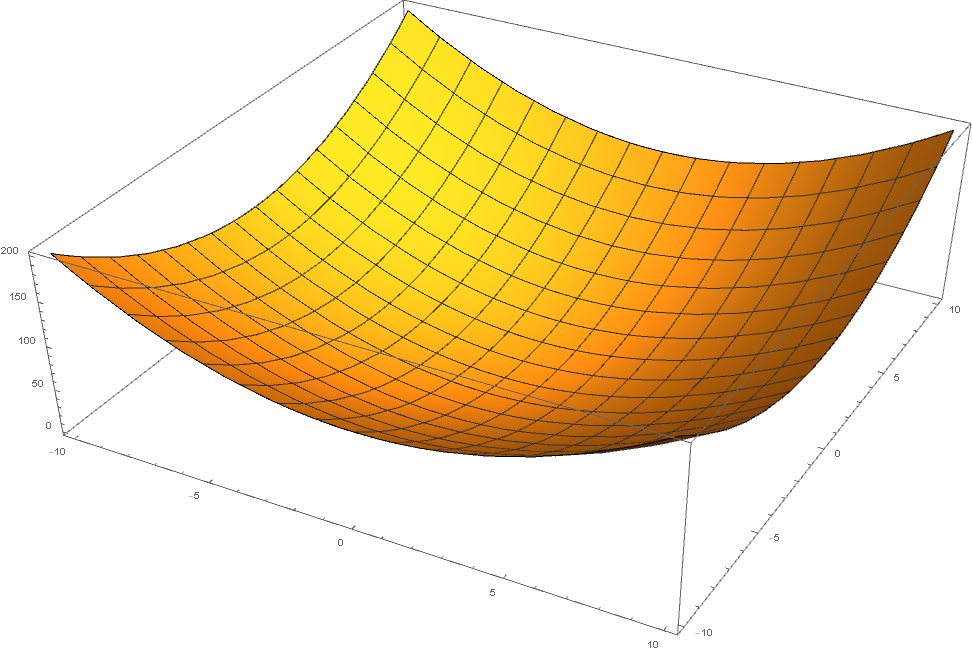
\includegraphics[height=7cm]{quadraticFunction1.png}\\
	\end{center}
	\caption{Funkcja kwadratowa dwóch parametrów}
\end{figure}

	\subsection{Funkcja Rastrigina}
	Funkcja Rastrigina jest funkcją ciągłą, skalowalną i multimodalną. Dzięki posiadaniu wielu minimum lokalnych, funkcja ta jest często stosowana w testowaniu algorytmów optymalizacyjnych. Przyjmuje ona następującą postać:

\[f(x) = An + \sum_{i=1}^{n} [x_i^2 - A \cos{(2 \pi x_i)}] \]

gdzie: \\
A = 10, \\
n = ilo\si ć wymiarów \\ \newLine

Warto\si ci tej funkcji są nieujemne. Zakres warto\si ci dla tej funkcji znajdziemy w przedziale:
\[x_i \in [-5.12, 5.12] \] \\

Posiada ona następujące globalne minimum:
\[ f(0,...,0) = 0 \] \\

By ujrzeć jej niektóre wła\si ciwo\si ci zaprezentowali\si my jej wykres w 2 wymiarach na poniższych obrazkach:\\
\begin{figure}[H]
	\begin{center}
		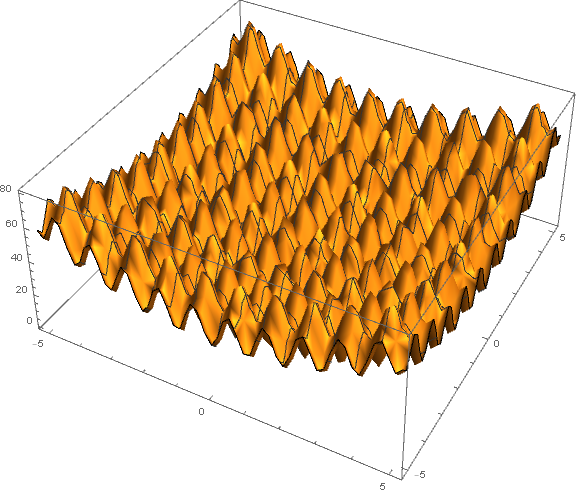
\includegraphics[height=7cm]{rastriginFunction1.png}\\
	\end{center}
	\caption{Funkcja Rastrigina o 2 wymiarach}
\end{figure}



	\subsection{Funkcja Rosenbrocka}
Funkcja ta jest funkcją ciągłą, skalowalną i jednomodalną.

\[f(x) = \sum_{i=1}^{n-1} [100(x_{i+1} - x_i^2)^2 + (1- x_i)^2 ]\] \\


Funkcja ta również przyjmuje wyłącznie warto\si ci nieujemne. Na potrzeby projektu warto\si ci argumentów dla tej funkcji zostały zawężone do poniższego zakresu:
\[x_i \in [-10, 10] \] \\

Posiada ona następujące globalne minimum:
\[ f(1,...,1) = 0 \] \\

Poniższe wykresy prezentują jej wygląd w zadanym zakresie:\\
\begin{figure}[H]
	\begin{center}
		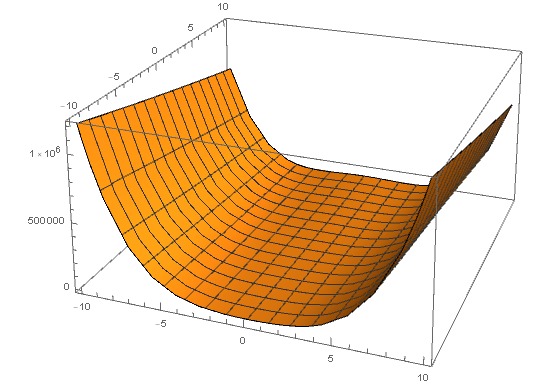
\includegraphics[height=7cm]{rosenbrockFunction1.png}\\
	\end{center}
	\caption{Funkcja Rosenbrocka o 2 wymiarach}
\end{figure}

\section{Dobór parametrów}
Pomimo, iż algorytmy heurystyczne są dobrym wyborem wszędzie tam, gdzie ważny jest czas znalezienia rozwiązania, to przed skorzystaniem z danego algorytmu jeste\si my zmuszeni ustawić parametry algorytmu w taki sposób, by wynik był dostatecznie dokładny, a algorytm nie wykonywał niepotrzebnie obliczeń, zwłaszcza gdy większa dokładno\si ć nie jest nam potrzebna lub nie będzie stanowić większej różnicy w stosunku do już znalezionego wyniku. Dodatkową trudno\si ć stanowi ilo\si ć parametrów oraz to, iż każdy z nich może wpływać w inny sposób na złożono\si ć obliczeniową oraz wynik, oraz parametry mogą być od siebie zależne. W opracowaniach naukowych rzadko kiedy można znaleźć wytyczne co do sposobu znalezienia odpowiednich parametrów do konkretnych problemów. \\

Starając się trzymać zasad dotyczących tworzenia dobrego algorytmu heurystycznego, przyjęli\si my kilka założeń, a następnie sukcesywnie poszukiwali\si my odpowiednich warto\si ci dla parametrów by (\si redni, 10-krotne powtórzenia) wynik był jak najlepszy, starając się zawężać zakres z czasem. Kiedy (\si rednie) wyniki były już zadowalające, sprawdzali\si my jako\si ć dobranych parametrów wykonując 100 razy algorytm z takimi samymi parametrami dla tego samego problemu, uzysując w prosty sposób procentową jako\si ć algorytmu. W podsekcji "Dobieranie parametrów dla funkcji 5 wymiarowej funkcji Rastrigina" tabele przedstawią stopniowe doj\si cie do parametrów dających zadowalające wyniki, a następnie jako\si ć tych parametrów dla danego problemu. Parametry dla innych problemów zostały zbadane w taki sam sposób i w tych sekcjach zostanie wspomniany jedynie wynik.

	\subsection{Dobieranie parametrów dla funkcji 5 wymiarowej funkcji Rastrigina}

Przed rozpoczęciem testów przyjęto dwa założenia:
\begin{enumerate}
	\item Końcowa temperatura została ustawiona na stałą warto\si ć równą 0.001,
	\item Stopień chłodzenia temperatury został ustawiony na 0.99.
\end{enumerate}

\renewcommand\arraystretch{1.333}


\begin{tabularx}{\textwidth}{ | >{\rownum}c|X|X|X|} 
\hline
& \textbf{ T0} & \textbf{ Iteracje} &\textbf{ Rozwiązanie}\\ \hline
& 500 & 300 & 1,09718505292704 \\ \hline 
& 500 & 400 & 1,29513703551228 \\ \hline 
& 100 & 500 & 1,29579688714116 \\ \hline 
& 300 & 400 & 1,39516546905179 \\ \hline 
& 100 & 400 & 1,59400704106305 \\ \hline 
& 400 & 200 & 1,59460563439097 \\ \hline 
& 400 & 400 & 1,59473245683331 \\ \hline 
& 300 & 500 & 1,69368418646326 \\ \hline 
& 100 & 200 & 1,69430049805511 \\ \hline 
& 400 & 500 & 1,69488738622795 \\ \hline 
& 200 & 500 & 1,79356181491557 \\ \hline 
& 500 & 200 & 1,89311831496136 \\ \hline 
& 300 & 100 & 1,89379034166828 \\ \hline 
& 200 & 200 & 1,89405233085409 \\ \hline 
& 400 & 300 & 1,99208845088035 \\ \hline 
& 500 & 500 & 1,99250333315708 \\ \hline 
& 300 & 300 & 1,99272286399703 \\ \hline 
& 200 & 400 & 2,09157445324622 \\ \hline 
& 100 & 300 & 2,19168206783873 \\ \hline 
& 300 & 200 & 2,19179918169512 \\ \hline 
& 500 & 100 & 2,19209302230291 \\ \hline 
& 200 & 100 & 2,19237079270076 \\ \hline 
& 400 & 100 & 2,19237108578013 \\ \hline 
& 200 & 300 & 2,29096718181202 \\ \hline 
& 100 & 100 & 2,98943206230488 \\ \hline 
\end{tabularx}

Badanie zawarte w tabeli 1 pokazuje, iz parametry na takim poziomie nie maja az tak duzego znaczenia, jednak mozna zauwazyc, iz wieksza wartosc parametrow prowadzi do nieco lepszych srednich wynikow.
Badanie skutecznosci dla najwyzszych parametrow (czyli 500 i 500) wynioslo 12\%, co jest bardzo slabym wynikiem.


\begin{tabularx}{\textwidth}{ | >{\rownum}c|X|X|X|} 
                 \hline
                 & \textbf{ T0}
                 & \textbf{ Iteracje}
                 &\textbf{ Rozwiązanie}\\ \hline
& 8000 & 6000 & 0,400456362305732 \\ \hline 
& 10000 & 4000 & 0,400942457997776 \\ \hline 
& 4000 & 8000 & 0,499468816488703 \\ \hline 
& 4000 & 10000 & 0,499496708877431 \\ \hline 
& 6000 & 6000 & 0,499881155483216 \\ \hline 
& 8000 & 8000 & 0,500190776858622 \\ \hline 
& 8000 & 10000 & 0,500669723808464 \\ \hline 
& 2000 & 6000 & 0,500802825547873 \\ \hline 
& 2000 & 4000 & 0,59876018888673 \\ \hline 
& 2000 & 8000 & 0,598944859155338 \\ \hline 
& 10000 & 8000 & 0,69839967735632 \\ \hline 
& 6000 & 8000 & 0,698671405088412 \\ \hline 
& 10000 & 10000 & 0,698922421188404 \\ \hline 
& 4000 & 6000 & 0,797834332682657 \\ \hline 
& 6000 & 10000 & 0,798499451192562 \\ \hline 
& 4000 & 4000 & 0,798596850008959 \\ \hline 
& 2000 & 10000 & 0,798896772938739 \\ \hline 
& 8000 & 4000 & 0,79899550599823 \\ \hline 
& 10000 & 6000 & 0,898177793387154 \\ \hline 
& 6000 & 4000 & 0,898733662378301 \\ \hline 
& 4000 & 2000 & 0,996463628047726 \\ \hline 
& 8000 & 2000 & 0,997870530143807 \\ \hline 
& 6000 & 2000 & 1,09703634442711 \\ \hline 
& 2000 & 2000 & 1,09731890136792 \\ \hline 
& 10000 & 2000 & 1,39564290923108 \\ \hline 
\end{tabularx}
10k i 10k
46\%\
5k - 10k -> 46\%
5k i 20k -> 58\%\
5k i 30k ->  72\%

\scalebox{0.5}{
\begin{tabularx}{\textwidth}{ | >{\rownum}c|X|X|X|}
  \hline
    & \textbf{T0} & \textbf{Iteracje} &\textbf{Rozwiązanie}\\ \hline
    & aaaaaaa aaaaaaa & aaaaaaa aaaaaaa  & oko\\ \hline
    & aaaaaaa aaaaaaa &aaaaaaa & oko \\ \hline
    & aaaaaaa & aaaaaaaaaaaaaa & oko \\ \hline
 & aaaaaaa & aaaaaaaaaaaaaa & oko \\ \hline
 & aaaaaaa & aaaaaaaaaaaaaa & oko \\ \hline
 & aaaaaaa & aaaaaaaaaaaaaa & oko \\ \hline
 & aaaaaaa & aaaaaaaaaaaaaa & oko \\ \hline
 & aaaaaaa & aaaaaaaaaaaaaa & oko \\ \hline
 & aaaaaaa & aaaaaaaaaaaaaa & oko \\ \hline
 & aaaaaaa & aaaaaaaaaaaaaa & oko \\ \hline
 & aaaaaaa & aaaaaaaaaaaaaa & oko \\ \hline
 & aaaaaaa & aaaaaaaaaaaaaa & oko \\ \hline
   & aaaaaaa aaaaaaa & aaaaaaa aaaaaaa  & oko\\ \hline
    & aaaaaaa aaaaaaa &aaaaaaa & oko \\ \hline
    & aaaaaaa & aaaaaaaaaaaaaa & oko \\ \hline
 & aaaaaaa & aaaaaaaaaaaaaa & oko \\ \hline
 & aaaaaaa & aaaaaaaaaaaaaa & oko \\ \hline
 & aaaaaaa & aaaaaaaaaaaaaa & oko \\ \hline
 & aaaaaaa & aaaaaaaaaaaaaa & oko \\ \hline
 & aaaaaaa & aaaaaaaaaaaaaa & oko \\ \hline
 & aaaaaaa & aaaaaaaaaaaaaa & oko \\ \hline
 & aaaaaaa & aaaaaaaaaaaaaa & oko \\ \hline
 & aaaaaaa & aaaaaaaaaaaaaa & oko \\ \hline
 & aaaaaaa & aaaaaaaaaaaaaa & oko \\ \hline
 & aaaaaaa & aaaaaaaaaaaaaa & oko \\ \hline
 & aaaaaaa & aaaaaaaaaaaaaa & oko \\ \hline
 & aaaaaaa & aaaaaaaaaaaaaa & oko \\ \hline
 & aaaaaaa & aaaaaaaaaaaaaa & oko \\ \hline
 & aaaaaaa & aaaaaaaaaaaaaa & oko \\ \hline
 & aaaaaaa & aaaaaaaaaaaaaa & oko \\ \hline
 & aaaaaaa & aaaaaaaaaaaaaa & oko \\ \hline
 & aaaaaaa & aaaaaaaaaaaaaa & oko \\ \hline
 & aaaaaaa & aaaaaaaaaaaaaa & oko \\ \hline

\end{tabularx}
}







\begin{tabularx}{\textwidth}{ | >{\rownum}c|X|X|X|}
  \hline
    & \textbf{T0} & \textbf{Iteracje} &\textbf{Rozwiązanie}\\ \hline
    & aaaaaaa aaaaaaa & aaaaaaa aaaaaaa  & oko\\ \hline
    & aaaaaaa aaaaaaa &aaaaaaa & oko \\ \hline
    & aaaaaaa & aaaaaaaaaaaaaa & oko \\ \hline
 & aaaaaaa & aaaaaaaaaaaaaa & oko \\ \hline
 & aaaaaaa & aaaaaaaaaaaaaa & oko \\ \hline
 & aaaaaaa & aaaaaaaaaaaaaa & oko \\ \hline
 & aaaaaaa & aaaaaaaaaaaaaa & oko \\ \hline
 & aaaaaaa & aaaaaaaaaaaaaa & oko \\ \hline
 & aaaaaaa & aaaaaaaaaaaaaa & oko \\ \hline
 & aaaaaaa & aaaaaaaaaaaaaa & oko \\ \hline
 & aaaaaaa & aaaaaaaaaaaaaa & oko \\ \hline
 & aaaaaaa & aaaaaaaaaaaaaa & oko \\ \hline

\end{tabularx}


\begin{tabularx}{\textwidth}{ | >{\rownum}c|X|X|X|}
  \hline
    & \textbf{T0} & \textbf{Iteracje} &\textbf{Rozwiązanie}\\ \hline
    & aaaaaaa aaaaaaa & aaaaaaa aaaaaaa  & oko\\ \hline
    & aaaaaaa aaaaaaa &aaaaaaa & oko \\ \hline
    & aaaaaaa & aaaaaaaaaaaaaa & oko \\ \hline
 & aaaaaaa & aaaaaaaaaaaaaa & oko \\ \hline
 & aaaaaaa & aaaaaaaaaaaaaa & oko \\ \hline
 & aaaaaaa & aaaaaaaaaaaaaa & oko \\ \hline
 & aaaaaaa & aaaaaaaaaaaaaa & oko \\ \hline
 & aaaaaaa & aaaaaaaaaaaaaa & oko \\ \hline
 & aaaaaaa & aaaaaaaaaaaaaa & oko \\ \hline
 & aaaaaaa & aaaaaaaaaaaaaa & oko \\ \hline
 & aaaaaaa & aaaaaaaaaaaaaa & oko \\ \hline
 & aaaaaaa & aaaaaaaaaaaaaa & oko \\ \hline

\end{tabularx}

Ostatecznie wybrane parametry dla tego problemu:\\
pocz temp\\
konc temp\\
cooling\\
iteracje\\

Badanie skutecznosci \\






skutecznosc:\\






	\subsection{Dobieranie parametrów dla funkcji 3 wymiarowej funkcji Rastrigina}
Ostatecznie wybrane parametry dla tego problemu:\\
pocz temp\\
konc temp\\
cooling\\
iteracje\\






skutecznosc:\\


	\subsection{Parametry dobrane dla funkcji kwadratowej dwóch parametrów}
Ostatecznie wybrane parametry dla tego problemu:\\
pocz temp\\
konc temp\\
cooling\\
iteracje\\






skutecznosc:\\

	\subsection{Parametry dobrane dla funkcji Rosenbrocka}
Ostatecznie wybrane parametry dla tego problemu:\\
pocz temp\\
konc temp\\
cooling\\
iteracje\\






skutecznosc:\\

\section{Implementacja}

Na realizację algorytmu symulowanego wyżarzania składa się implementacja kilku metod, które zostały przedstawione w roździale 2.1.2 i będą tutaj omówione i/lub zostanie przedstawiony ich kod. \\

\subsection{Używane parametry i zmienne}
Wraz z zainicjalizowaniem obiektu symulowanego wyżarzania, ustawianych jest kilka parametrów na wej\si cie, a konkretniej problem do rozwiązania i parametry samego algorytmu. W moim programie nazywane są: \textbf{Function}, \textbf{Arguments}, \textbf{Arguments2}, \textbf{Iterations}, \textbf{BeginingTemperature}, \textbf{EndingTemperature}, \textbf{Cooling}, \textbf{SatisfactionSolutionValue}. \\

\textbf{Function} jest identyfikatorem referencji do obiektu problemu. Każdy problem musi dziedziczyć po klasie abstrakcyjnej ,,TestingFunction", co zapewnia uniwersalno\si ć stosowania algorytmu symulowanego wyżarzania oraz zapewnia nasz algorytm, iż implementacja samego problemu będzie posiadać pewne cechy (jak np. jawnie okre\si loną ilo\si ć wymiarów). \\

\textbf{Arguments} jest wła\si ciwo\si cią w postaci tablicy liczb zmiennoprzecinkowych, które zawierają argumenty dla obecnie najlepszego rozwiązania problemu. \\

\textbf{Arguments2} jest również tablicą liczb zmiennoprzecinkowych, jednak przechowuje ona warto\si ci argumentów dla tymczasowego rozwiązania. Jest tego samego rozmiaru, co wła\si ciwo\si ć \textbf{Arguments}. \\

\textbf{Iterations} jest liczbą wewnętrznych iteracji. Tyle razy algorytm będzie szukał sąsiadów najlepszego rozwiązania, zanim obniży temperaturę. \\

\textbf{BeginingTemperature} jest to początkowa warto\si ć temperatury, od której rozpoczyna się proces poszukiwań rozwiązania. \\ 

\textbf{EndingTemperature} jest liczbą, którą obniżana temperatura (zmienna \textbf{temperature}) musi osiągnąć, by zakończyć działanie algorytmu. \\

\textbf{Cooling} to liczba zmiennoprzecinkowa, w każdym globalnym kroku algorytmu zmienna \textbf{temperature} jest mnożona przez tą warto\si ć. Jest ona mniejsza od 1, więc temperatura powoli się obniża. \\

\textbf{SatisfactionSolutionValue} jest minimalną liczbą, jaką rozwiązanie musi osiągnąć, aby wynik poszukiwania rozwiązania był dla satysfakcjonujący. Jest to zmienna opcjonalna, algorytm nadal będzie działać, gdy nie poda się jej warto\si ci.\\

W programie również używam kilku pomocnicznych zmiennych: \\

\textbf{temperature} to zmienna, która przetrzymuje obecną liczbę stanowiącą temperaturę. Jest ona używana przy warunkach globalnej iteracji oraz przy funkcji prawdopodobieństwa. Wraz z postępem iteracji maleje. \\

\textbf{bestSolution} to liczba zmiennoprzecinkowa, która jest obecnie najlepszym wynikiem rozwiązania. Finalnie będzie ona najlepszym rozwiązaniem całego problemu. \\

\textbf{tmpSolution} jest tymczasowym wynikiem rozwiązania (wynikiem rozwiązania problemu dla parametrów ze zmiennej \textbf{Arguments2}). \\

\textbf{counter} jest liczbą oznaczającą obecną, globalną iterację. \\

\subsection{Schemat blokowy}
Przygotowali\si my również schemat blokowy reprezentujący poszczególne kroki i scenariusze w procesie poszukiwania rozwiązania zadanego problemu, co można zobaczyć na poniższym rysunku.

\begin{figure}[H]
		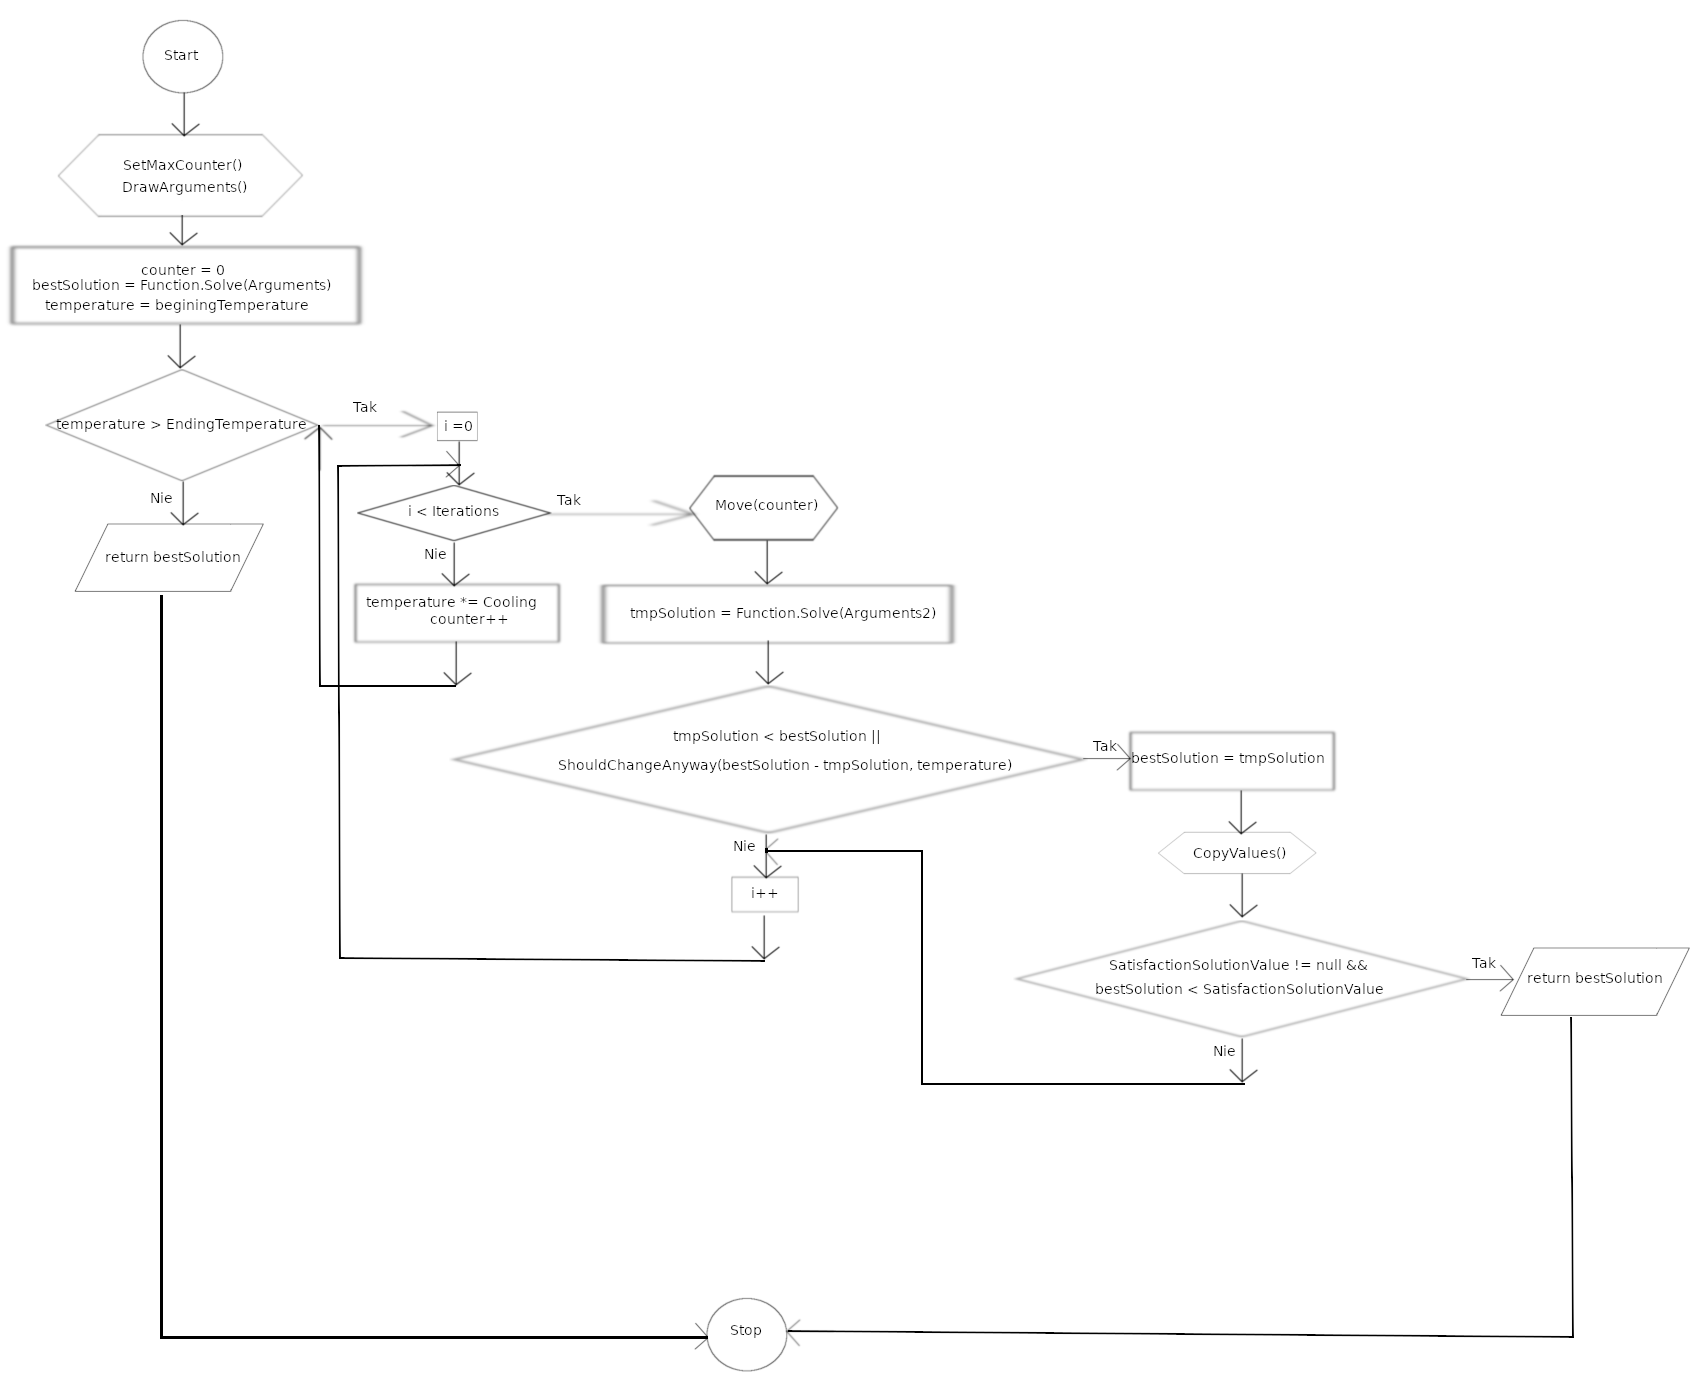
\includegraphics[height=22cm, width=16cm]{schematBlokowy.png}\\
	\caption{Schemat blokowy algorytmu symulowanego wyżarzania}
\end{figure}

\subsection{Implementacja metod i algorytmu}

\underline{Funkcja SetMaxCounter()} \\
Metoda ta symuluje proces obniżania temperatury w celu obliczenia maksymalnej ilo\si ci globalnych iteracji. \\
\begin{verbatim}
private void SetMaxCounter()
{
    maxCounter = 0;
    double tmpTemperature = BeginingTemperature;
    while (tmpTemperature > EndingTemperature)
    {
        tmpTemperature *= Cooling;
        maxCounter++;
    }
}
\end{verbatim}

\underline{Funkcja DrawArguments()} \\
W metodzie tej losuję początkowe argumenty (wła\si ciwo\si ć \textbf{Arguments}) z przedziału zadanego w danym problemie. \\

\underline{Funkcja Move()} \\
W tym kroku najpierw obliczany jest pozostały procent iteracji do ukończenia procesu. Następnie biorąc 80\% pełnej puli możliwych warto\si ci problemu, mnożymy ją przez pozostały procent iteracji (i przypisujemy do zmiennej value). Dalej, w pętli, każdemu argumentowi tymczasowego rozwiązania (wła\si ciwo\si ć \textbf{Arguments2}), przypisywana jest suma odpowiedniego argumentu najlepszego rozwiązania (aby był to sąsiad najlepszego rozwiązania) oraz losowa liczba z przedziału [-value, value]. Wraz z postępem iteracji zakres ten jest coraz węższy, ale rozwiązanie powinno też już być bliskie optymalnemu. Na końcu walidujemy nowy argument do podanego zakresu. \\
\begin{verbatim}
private void Move(int counter)
{
    double leftTemperatureCoolingTimes = maxCounter - counter;
    double leftPercent = leftTemperatureCoolingTimes / maxCounter;

    double domainValue = (Function.RightBound - Function.LeftBound);
    double value = (0.8 * domainValue) * (leftPercent);
    for (int i = 0; i < AmountOfArguments; i++)
    {
        double newValue = Arguments[i] + 
RandomGenerator.Instance.GetRandomDoubleInDomain(-value, value);
        if (newValue < Function.LeftBound)
        {
            newValue = Function.LeftBound;
        }
        if (newValue > Function.RightBound)
        {
            newValue = Function.RightBound;
        }
        Arguments2[i] = newValue;
    }
}
\end{verbatim}

\underline{Funkcja ShouldChangeAnyway()} \\
Jest to prosta implementacja funkcji prawdopodobieństwa, o której mowa była w rozdziale 2.1.1. \\

\underline{Funkcja CopyValues()} \\
Ze względu, iż język C\# traktuje tablicę jako obiekt, to tablica jest typem referencyjnym i konieczne jest skopiowanie warto\si ci ze zmiennej \textbf{Arguments2} do zmiennej \textbf{Arguments}. \\

\underline{Implementacja algorytmu} \\
Opisane metody są wykorzystywane w poszczególnych krokach samego algorytmu. Po obliczeniu maksymalnej ilo\si ci iteracji, algorytm losuje pierwsze rozwiązanie. Następnie w pętli i następnej zagnieżdzonej pętli, szuka sąsiada obecnego najlepszego rozwiązania. Zamienia nowe rozwiązanie ze starym jeżeli zostały spełnione odpowiednie warunki. Jeżeli nowe rozwiązanie spełnia kolejny warunek, to kończy program zwracając najlepsze rozwiązanie. Jeżeli nie, wychodzi z zagnieżdzonej pętli, zmniejsza zmienną odpowiedzialną za temperaturę i jest to koniec kroków w jednej pełnej, ,,globalnej" iteracji. Jeżeli program nie osiągnie satysfakcjonującego rozwiązania, a proces obniżania temperatury zakończy się, zwróci rozwiązanie, które udało mu się znaleźć kończąc tym samym program.

\begin{verbatim}
public double Solve()
{
    SetMaxCounter();
    int counter = 0;

    DrawArguments();
    double bestSolution = Function.Solve(Arguments);

    double temperature = BeginingTemperature;
    while (temperature > EndingTemperature)
    {
        for (int i = 0; i < Iterations; i++)
        {
            Move(counter);
            double tmpSolution = Function.Solve(Arguments2);

            if (tmpSolution < bestSolution || 
ShouldChangeAnyway(bestSolution - tmpSolution, temperature))
            {
                bestSolution = tmpSolution;
                CopyValues();
                if(SatisfactionSolutionValue != null &&
 bestSolution < SatisfactionSolutionValue)
                {
                    return bestSolution;
                }
            }
        }
        temperature *= Cooling;
        counter++;
    }
    return bestSolution;
}
\end{verbatim}

\section{Zastosowanie algorytmów w rozwiązywaniu odwrotnego zagadnienia przewodnictwa ciepła}
\section{Narzędzia i technologie}
	\subsection{Metodyka pracy}
	\subsubsection{System kontroli wersji}
	System kontroli wersji posiada wiele zalet, m.in.: bezpieczeństwo, możliwo\si ć pracy w kilku miejscach/urządzeniach nad tym samym problemem, łatwą możliwo\si ć przywrócenia poprzedniej wersji, czy wreszcie, inspekcję jako\si ci i poprawno\si ci kodu. \\
W moim projekcie skorzystałem z systemu kontroli Git, a repozytorium można znaleźć na portalu github.com. 
	\subsubsection{Github Project Management}
Pomimo, iż praca w pojedynkę nie wymagała ode mnie zaawansowanego zarządzania projektem i konieczno\si ci organizacji pracy, zdecydowałem się na użycie narzędzia pozwalającego na taką pracę. Podzielenie projektu na mniejsze zadania pozwoliło mi wydzielić poszczególne i odrębne sektory pracy, widzieć postępujący progres i łatwo odnaleźć się w aktualnie wykonywanym zadaniu. W tym celu skorzystałem z Github Project Management, który pozwala na proste zarządzanie zadaniami.
	\subsubsection{\SI rodowisko programistyczne}
Do implementacji projektu użyłem \si rodowiska Microsoft Visual Studio Community 2017, które to zostało stworzone przez firmę Microsoft i pozwala na programowanie konsolowe oraz z graficznym interfejsem użytkownika (zarówno aplikacje desktopowe, jak i strony internetowe).  \\
Dobra znajomo\si ć i przejrzysto\si ć tego \si rodowiska programistycznego pozwoliła mi skupić się na rozwiązywaniu problemu, omijając problem zapoznawania się z nowym narzędziem.
	\subsubsection{Mathematica}
	Mathematica jest programem opartym na systemie obliczeń symbolicznych oraz numerycznych. Program ten jest do\si ć popularny w\si ród naukowców ze względu na wiele zalet, jak np. wydajno\si ć czy rozpięte możliwo\si ci wizualizacji danych. Mathematica jest programem komercyjnym, dlatego stworzenie wykresów do tego projektu oparłem na licencji wydziału Matematyki Stosowanej.
	
	\subsection{Użyte technologie}
	\subsubsection{C\#}
Język programowania C\# należy do obiektowych języków programowania, którego koncepcja opiera się na tworzeniu klas, które poprzez swoją zawarto\si ć (m.in. wła\si ciwo\si ci czy metody) mogą być reprezentowane poprzez obiekty i każde operacje są wykonywane poprzez nie. W projekcie korzystam z języka C\# w wersji 7.0, która w momencie rozpoczęcia pracy była aktualna. Dobra znajomo\si ć tego języka pozwoliła mi nie zważać na problemy w znajomo\si ci składni czy funkcji i skupić się bezpo\si rednio na implementacji algorytmów, dobraniu odpowiednich parametrów dla poszczególnych funkcji testowych oraz lepszym przetestowaniu całej funkcjonalno\si ci.

\subsubsection{Wolfram Language}
Język ten służy głównie do programowania obliczeń matematycznych i programowania funkcjonalnego w programie Mathematica. Język ten, wraz z oprogramowaniem Mathematica, pozwalają m.in. na: operacje na macierzach, rozwiązywanie równań różniczkowych czy prezentowanie danych za pomocą wykresów. Z tej ostatniej funkcjonalno\si ci skorzystałem tworząc wykresy funkcji testowych.

\section{Podsumowanie}
	\subsection{Dalsze kierunki rozwoju}
	\subsection{Źródła}
%funkcje testowe
https://www.ncbi.nlm.nih.gov/pmc/articles/PMC4538776/

%wstep i opis problemu[?]
F. Rothlauf, Design of Modern Heuristics, Natural Computing Series,
DOI 10.1007/978-3-540-72962-4 2, © Springer-Verlag Berlin Heidelberg 2011

%wstep i opis problemu
R. Mart'ı and G. Reinelt, The Linear Ordering Problem, Exact and Heuristic Methods
in Combinatorial Optimization 175, DOI: 10.1007/978-3-642-16729-4 2,
c Springer-Verlag Berlin Heidelberg 2011

%problemy odwrotne/1 rozdzial
http://prac.im.pwr.edu.pl/~plociniczak/lib/exe/fetch.php?media=odwrotne.pdf

https://www.math.unl.edu/~scohn1/8423/wellposed.pdf

%


----------------------------------------------------------------------------------------------------------------------

\begin{thebibliography}{12}

\bibitem{PozNazwa1} Jakaś pozycja literatury
\bibitem{InnPoz} Jakaś pozycja literatury

\end{thebibliography}
\end{document}
